\documentclass[10pt, aspectratio=169, usepdftitle=false]{beamer}

\usetheme[progressbar=frametitle]{metropolis}
% \usecolortheme{beaver}
% \usecolortheme{fly}
% \usecolortheme{beetle}
\usepackage{appendixnumberbeamer} % Probably not needed
\usepackage[danish]{babel}
\usepackage{hyperref} %References
\hypersetup{
    pdftitle={SOP 2019 --- Præsentation},
    pdfauthor={Jens Tinggaard}
}

\usepackage{booktabs} % what is this?
\usepackage[scale=2]{ccicons} % and this?

\usepackage{pgfplots} % Do i need this?
\usepgfplotslibrary{dateplot}

\usepackage{xspace} % Or this?

% \let\textttorig\texttt
% \renewcommand<>{\texttt}[1]{%
%   \only#2{\textttorig{#1}}%
% }
\title{Studieområdeprojekt 2019}
\subtitle{Sikkerhed bag login-formular på en hjemmeside}
\date{27. januar 2020}
\author{Jens Tinggaard}
\institute{Odense Tekniske Gymnasium}
\titlegraphic{\hfill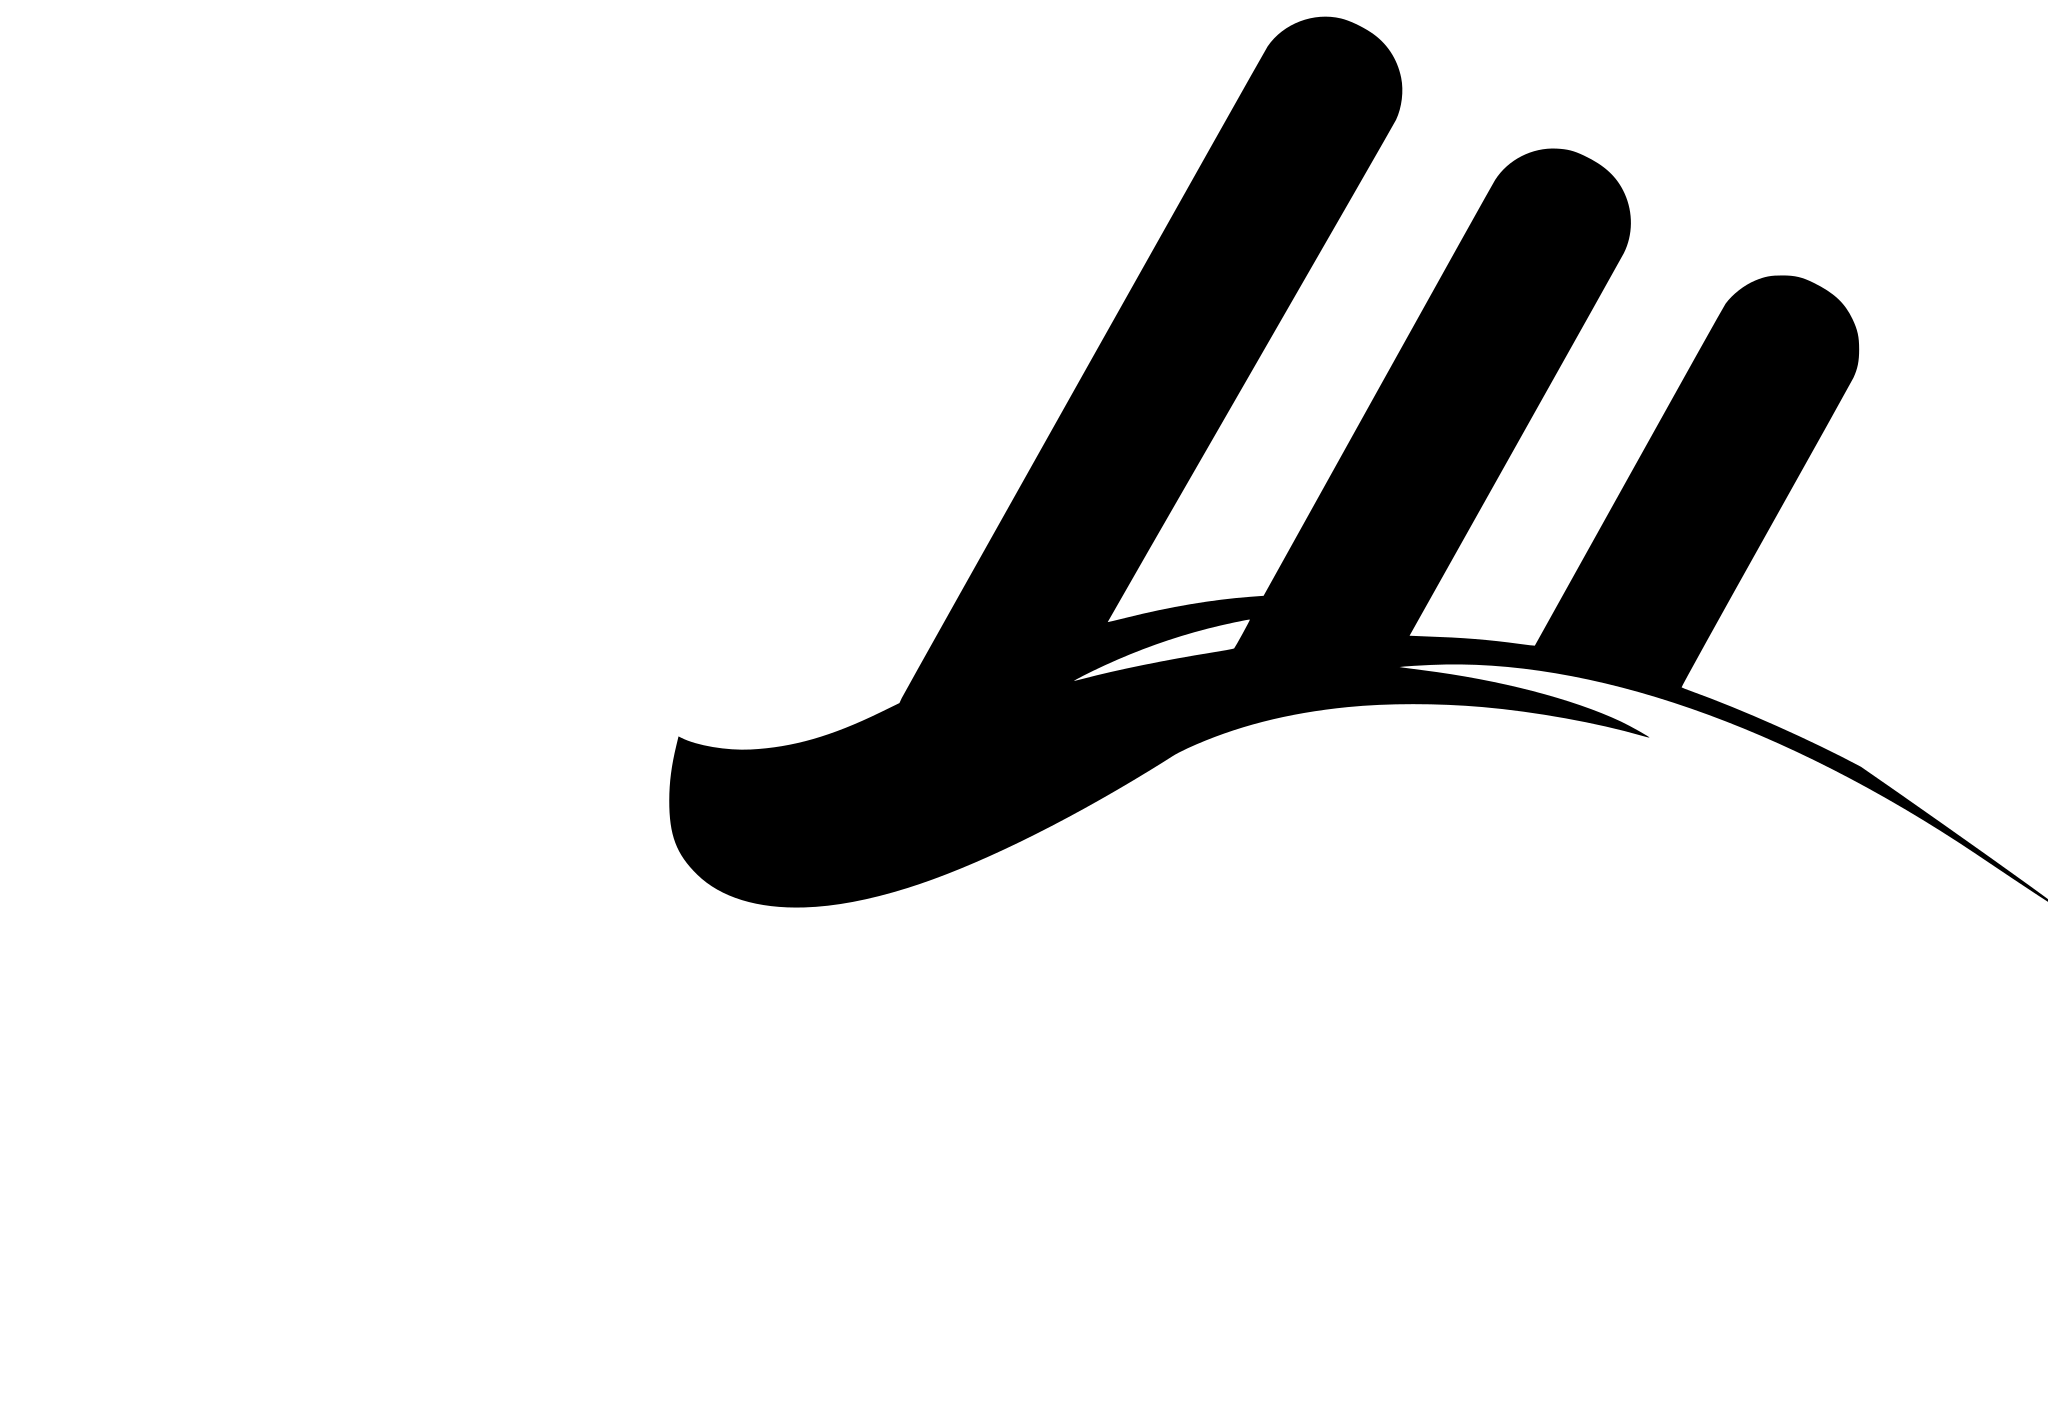
\includegraphics[height=1.5cm]{img/otg_logo.png}}



\begin{document}

\maketitle


\begin{frame}{Opgaveformulering}
\begin{itemize}
    \large
    \item Redegør for talteorien bag RSA kryptering. Forklar nødvendigheden af primtal og hvordan RSA metoden fungerer.
    \item Gør kort rede for hashing.
    \item Analyser forskellen på hashing og kryptografi og hvilken rolle de har i forhold til sikkerhed.
    \item Vurder hvorfor RSA er vigtigt i forbindelse med sikkerhed ved logins.
\end{itemize}
\end{frame}
%--- Next Frame ---%

\begin{frame}{Konklusion på projektet}
    \begin{itemize}
        \large
        \item Hvorfor er RSA så vigtig - hvor bruges det?
        \item Hvad RSA bygger på.
        \item Metoder som RSA og hashing bliver sjælendt brugt alene.
    \end{itemize}
\end{frame}
%--- Next Frame ---%

\section{SOP som metodefag}

\begin{frame}{Relevante metoder i fagene}
    \begin{columns}[T,onlytextwidth]
        \column{0.5\textwidth}
            \alert{Matematik:}
            \begin{enumerate}
                \item Talteori.
                \item Beviser. %\(\qed\)
                \item Vurdering \& Sammenligninger.
            \end{enumerate}
        \column{0.5\textwidth}
            \alert{Programmering:}
            \begin{enumerate}
                \item Prototkoller.
                \item Skitsering af id\'eer.
                \item Dokumentationslæsning.
            \end{enumerate}
    \end{columns}
\end{frame}
%--- Next Frame ---%


\begin{frame}{Empiri}
    \alert{Empiri brugt til udarbejdelse af projektet.}
    \begin{itemize}
        \item Litteratur.
        \item Dokumentation af programmer som \texttt{hashcat} og \texttt{gpg}.
        \item Standarder og protokoller til håndtering af disse.
        \item Virkelighedsdata som UNI-login.
    \end{itemize}
\end{frame}
%--- Next Frame ---%

\begin{frame}{Sammenspil mellem fagene}
    \alert{Sammenspil mellem fagene}
    \begin{itemize}
        \item Logisk tankegang.
        \item Protokol \(\rightarrow\) matematisk fremgangsmåde.
        \item Anvendt matematik \(\rightarrow\) programmering.
    \end{itemize}
\end{frame}
%--- Next Frame ---%

\begin{frame}{Kildekritik}
    \alert{Hvordan jeg har forholdt mig kildekritisk.}
    \begin{itemize}
        \item Bøger.
        \item Udgivet materiale.
        \item Pålidelig dokumentation.
    \end{itemize}
\end{frame}
%--- Next Frame ---%

\end{document}
